\documentclass[11pt]{article}
\usepackage[margin=1.5in]{geometry}
\usepackage{graphicx}
\usepackage{float}
\usepackage{parskip}
\usepackage{amsmath}
\usepackage{subfigure}
\usepackage{ulem}
\usepackage{pgfplots}
\usepackage{gensymb}
\pgfplotsset{width=10cm, compat=1.9}

\begin{document}

\textbf{\Huge Introduction to Trigonometry}

Athan Zhang \& Jeffrey Chen

\section{Right Triangle Trigonometry}
Trigonometry refers to the study of the ratios of side lengths in the context of right triangles. There are three basic trigonometric ratios:

\begin{figure}[H]
    \centering
    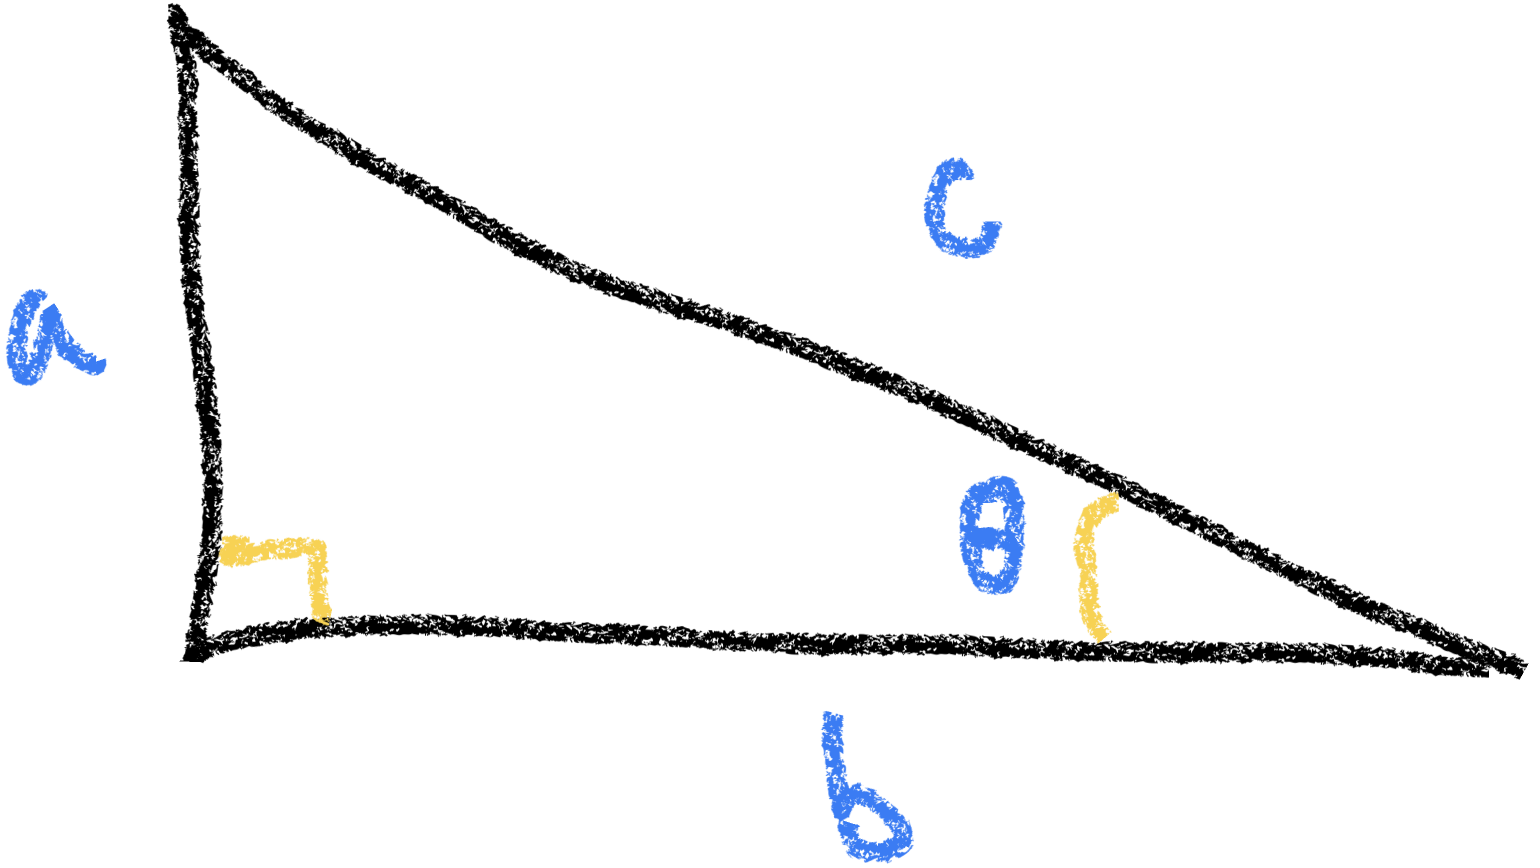
\includegraphics[width=0.5\textwidth]{Precalc/images/triangle.png}
    \caption{Right Triangle}
    \label{fig:triangle}
\end{figure}

\begin{enumerate}
    \item \textbf{Sine}: The sine of an angle is the ratio of the \textbf{opposite} side length over the \textbf{hypotenuse} length. For example, in the figure above, the sine of the angle $\theta$, written as $\sin(\theta)$, would be equal to $\frac{a}{c}$. The reciprocal of sine is known as the \textbf{cosecant}, and is written as $\csc(\theta)$.
    \item \textbf{Cosine}: The cosine of an angle is the ratio of the \textbf{adjacent} side length over the \textbf{hypotenuse} length. For example, in the figure above, the cosine of the angle $\theta$, written as $\cos(\theta)$, would be equal to $\frac{b}{c}$.The reciprocal of cosine is known as the \textbf{secant}, and is written as $\sec(\theta)$.
    \item \textbf{Tangent}: The tangent of an angle is the ratio of the \textbf{opposite} side length over the \textbf{adjacent} side length. For example, in the figure above, the tangent of the angle $\theta$, written as $\tan(\theta)$, would be equal to $\frac{a}{b}$. Note that the tangent is also equal to the sine over cosine. The reciprocal of tangent is known as the \textbf{cotangent}, and is written as $\cot(\theta)$.
\end{enumerate}

For example, the sine of $30\degree$ is equal to the ratio of the opposite side over the hypotenuse length in any right triangle with angle measure $30\degree$. This is visualized below:

\begin{figure}[H]
    \centering
    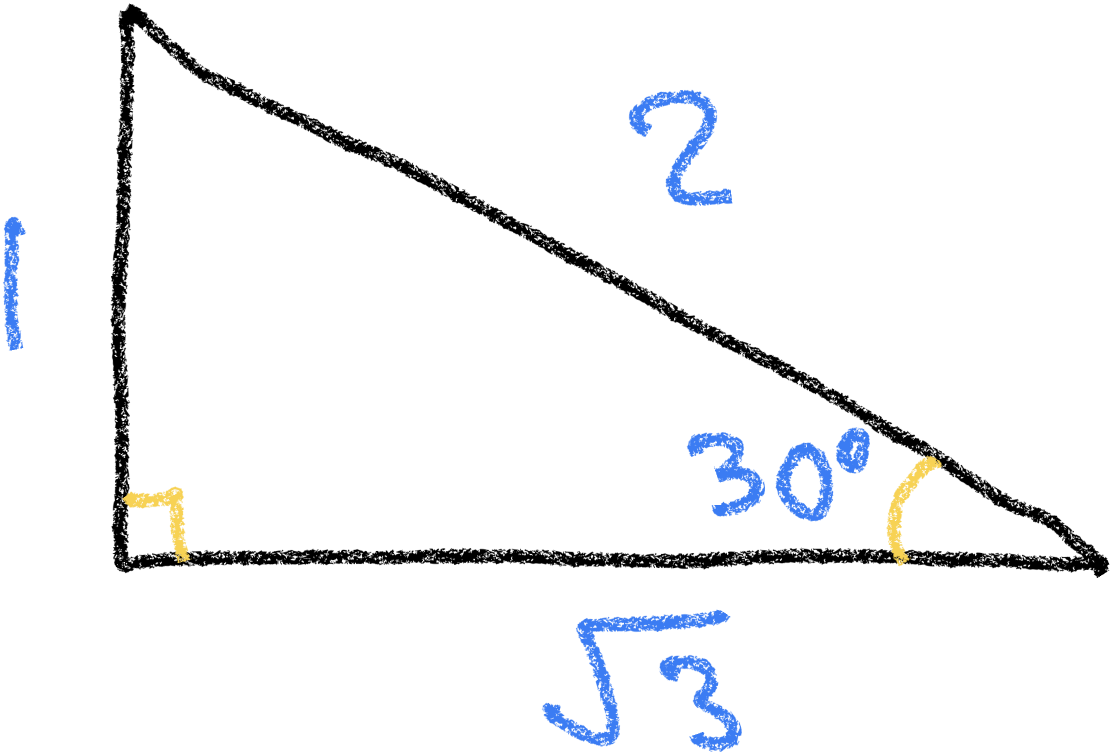
\includegraphics[width=0.5\textwidth]{Precalc/images/triangle2.png}
    \caption{Right Triangle With $30\degree$ Angle}
    \label{fig:triangle2}
\end{figure}

Therefore, the sine of $30\degree$ is $\frac{1}{2}$. Note that the actual side lengths do not matter; the ratios of side lengths stay the same regardless of how the triangle is scaled.


\section{Degrees and Radians}

 In trigonometry, degrees and radians are two different units of measuring angles. They provide a way to quantify and compare the magnitude of angles.

\subsection{Angles}

From geometry, you know that when two rays share a similar vertex, they form an angle. There is the initial side and terminal side. When an angle has its vertex at the origin of a Cartesian plane with one ray along the x-axis, it is considered to be in \textbf{standard position}.

An angle describes the amount of rotation necessary to move from the initial side to the terminal side. An angle can be positive (clockwise) or negative (counterclockwise). Figure \ref{fig:angles} illustrates this concept.

\begin{figure}[H]
    \centering
    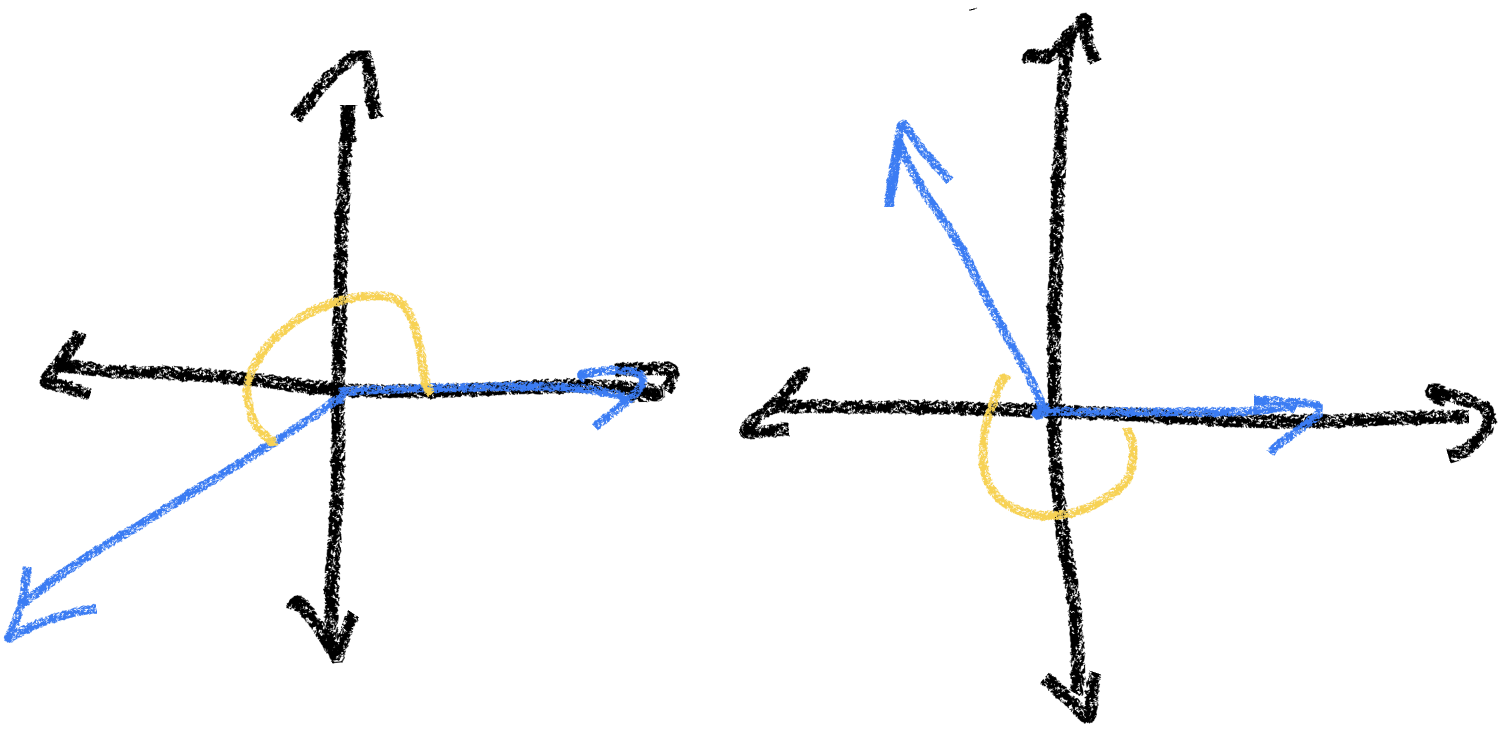
\includegraphics[width=0.7\textwidth]{Precalc/images/angles.png}
    \caption{(left) Positive Angle Drawing (right) Negative Angle Drawing}
    \label{fig:angles}
\end{figure}

\subsection{Degrees}

Degrees are the most common unit of angle measurement in everyday life. The concept of degrees is based on dividing a circle into 360 equal parts, with each part representing one degree ($^\circ$). A full circle is considered to be 360 degrees. Each degree can be further subdivided into minutes (') and seconds ("). One degree is equal to 60 minutes, and one minute is equal to 60 seconds.

For example, if you have an angle of 45 degrees, it means that the angle subtends one-forty-fifth (1/45) of a complete revolution or circle.

\subsection{Radians}

Radians are an alternative unit of measuring angles, particularly favored in mathematics and scientific applications. Unlike degrees, radians are based on the ratio of the arc length to the radius of a circle. Specifically, one radian (rad) is defined as the angle subtended at the center of a circle by an arc whose length is equal to the circle's radius.

Unlike degrees, which are measured from an arbitrary 360 degrees, radians are calculated as a ratio of lengths. Since radians are based on the relationship between the arc length and the radius, they are considered a more natural unit for measuring angles in mathematics. Many mathematical formulas and trigonometric identities are more straightforward and more elegant when angles are expressed in radians.

\textbf{Conversion between Degrees and Radians}

Radians to Degrees: Multiply by $\frac{180^\circ}{\pi\text{ radians}}$

Degrees to Radians: Multiply by $\frac{\pi\text{ radians}}{180^\circ}$

\textbf{Area of a Sector}

\begin{align*}
    \frac{A}{\pi r^2} &= \frac{\text{Arc length}}{2\pi r} \\
    \frac{A}{\pi r^2} &= \frac{r\theta}{2\pi r} \\  
    A &= \frac{1}{2}r^2 \theta
\end{align*}

\section{Unit Circle Trigonometry}

\subsection{Trigonometric Ratios of Any Angle}
So far, we have learned how to determine trigonometric ratios of positive acute angles. But what about obtuse and/or negative angles? This can be accomplished by drawing axes, tracing the angle counterclockwise, and drawing a vertical line either up or down to the x-axis to form a right triangle. This is visualized below:

\begin{figure}[H]
    \centering
    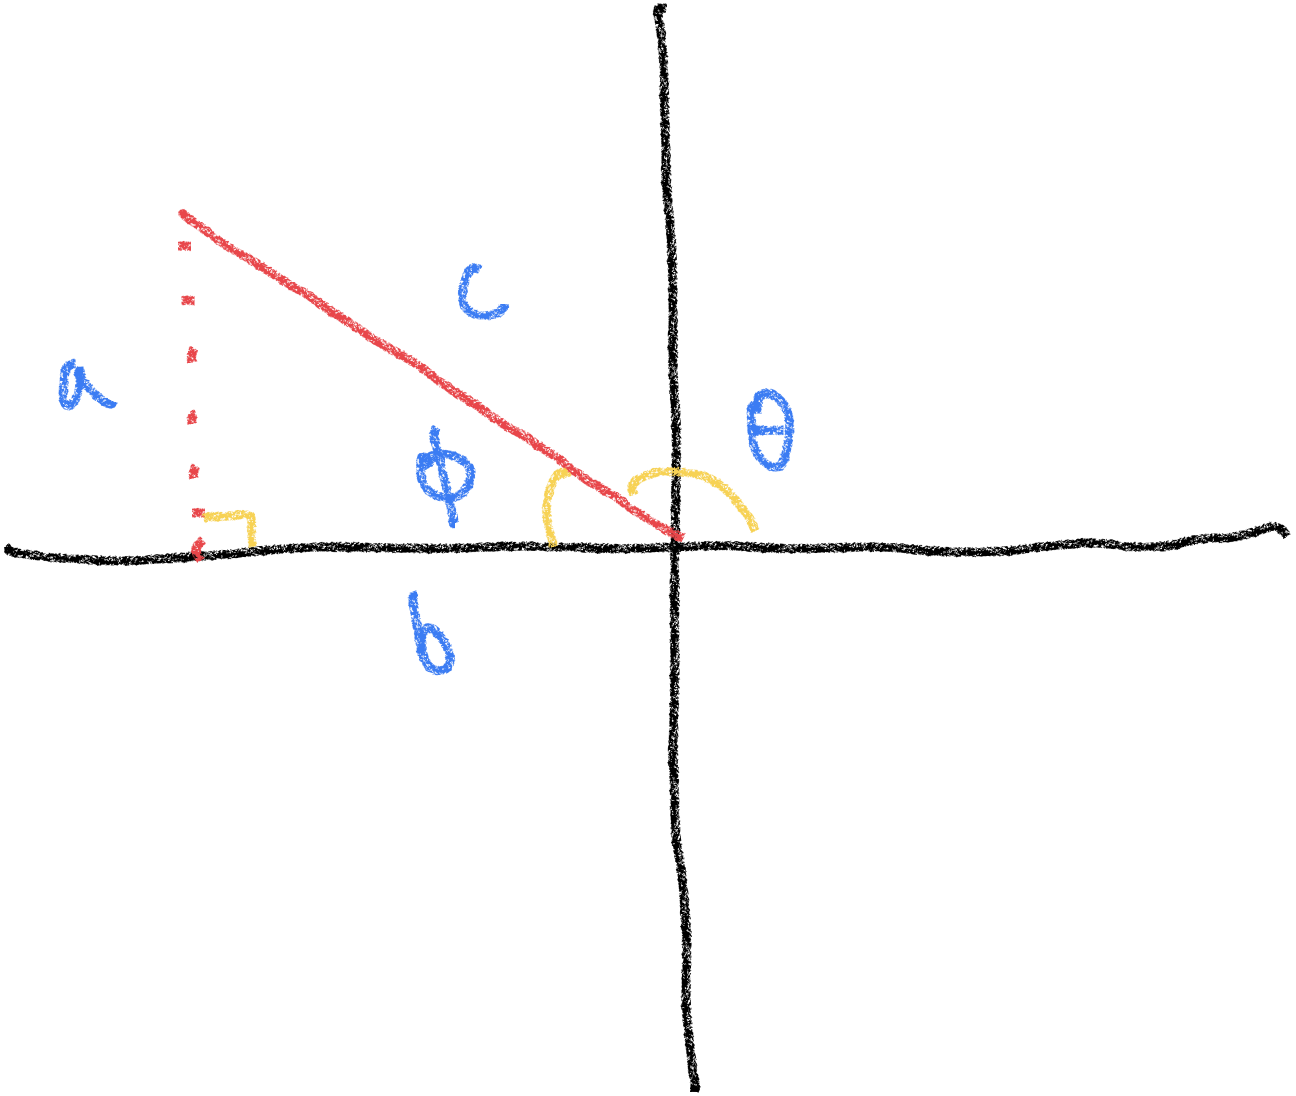
\includegraphics[width=0.5\textwidth]{Precalc/images/obtuse.png}
    \caption{Obtuse Angle Trigonometry}
    \label{fig:obtuse}
\end{figure}

As can be seen, the obtuse angle $\theta$ "creates" a right triangle that lies outside of the first quadrant with angle $\phi$. We call $\phi$ the \textbf{reference angle} of $\theta$. The \textbf{absolute value} of any trigonometric function of $\theta$ and $\phi$ are equal. The \textbf{sign} of the value of the function for $\theta$ is determined by the quadrant the angle lies in. For example, the sine of $\theta$ in this case would be equal to $\frac{a}{c}$, and the cosine would be equal to $-\frac{b}{c}$.

\subsection{The Unit Circle}
The \textbf{unit circle} is a circle of radius $1$ centered at the origin. Notice that given any radius with angle $\theta$ counterclockwise from the positive x-axis, we can draw a right triangle with the x-axis similar to the previous section, visualized below:



\begin{figure}[H]
    \centering
    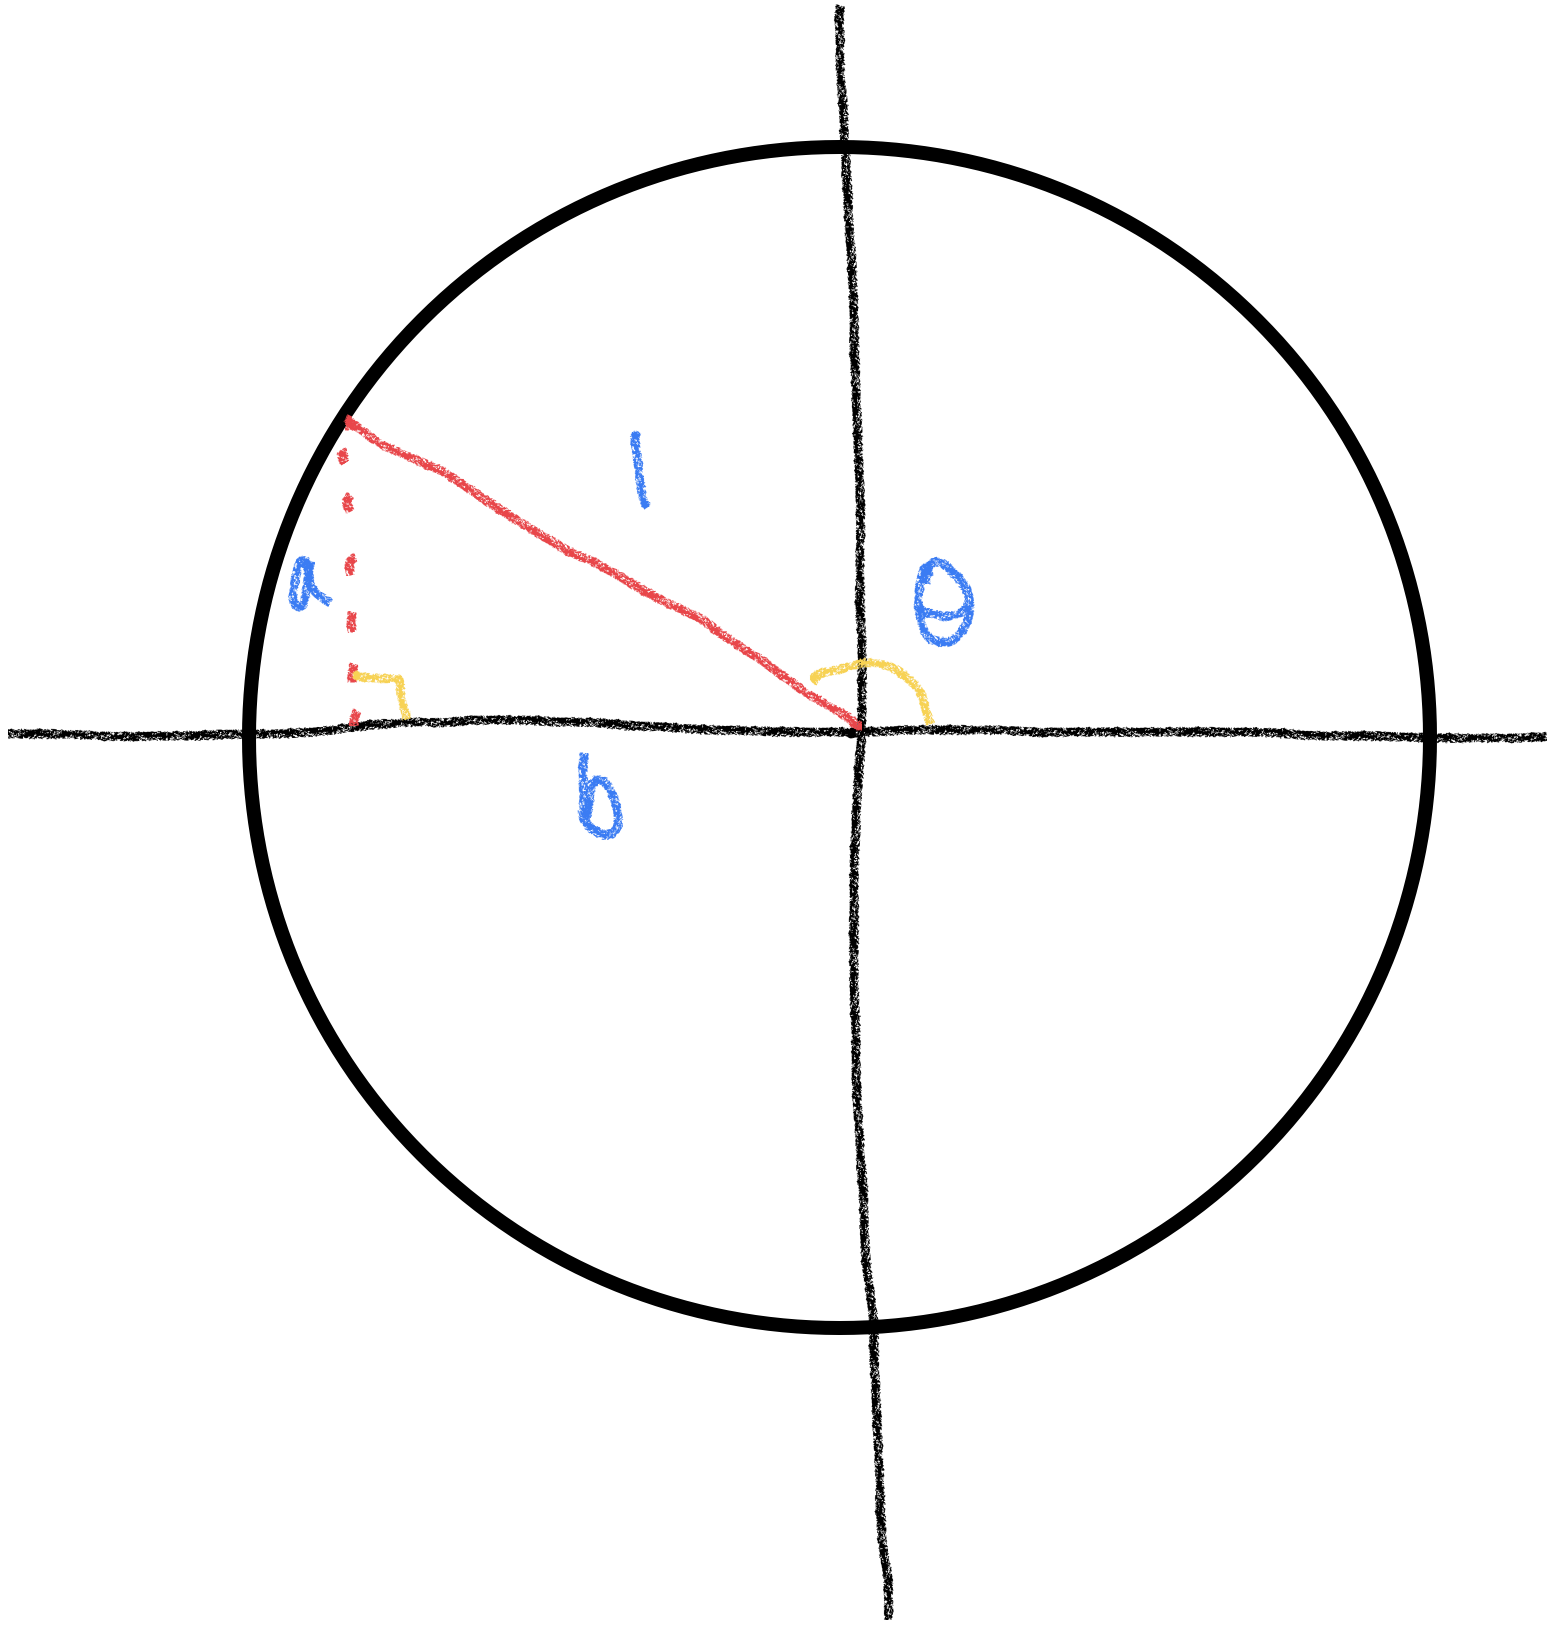
\includegraphics[width=0.5\textwidth]{Precalc/images/unitcircle.png}
    \caption{Obtuse Angle on the Unit Circle}
    \label{fig:unitcircle}
\end{figure}


The resulting right triangle always has hypotenuse length $1$. Thus, the unit circle is extremely useful for visualizing trigonometric ratios. Below is a complete $16$-point unit circle labeled with trigonometric ratios. These $16$ points are common angles that are extremely useful when mastered and memorized.

\begin{figure}[H]
    \centering
    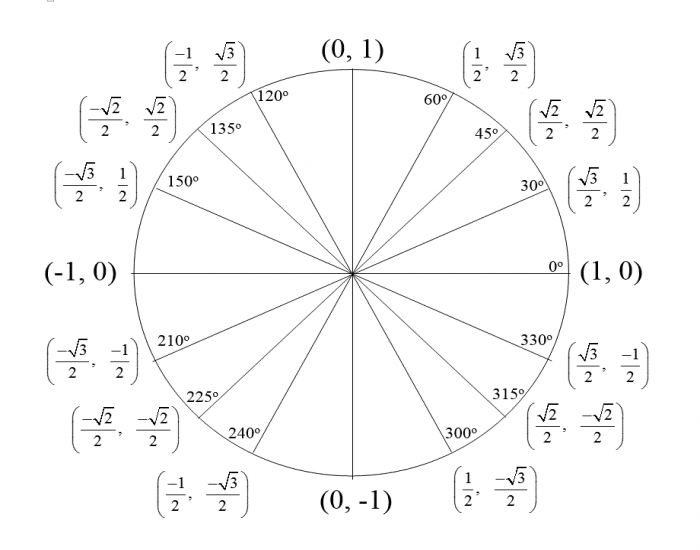
\includegraphics[width=0.7\textwidth]{Precalc/images/16pt.png}
    \caption{16 Point Unit Circle}
    \label{fig:16pt}
\end{figure}

\section{Graphing Trigonometric Functions}

\subsection{The Parent Functions}

The sine and cosine functions are \textbf{cyclic}, as can be observed from the unit circle. This means that their behavior repeats over a set \textbf{period}. The period of $\sin x$ and $\cos x$ is $2\pi$. Both $\sin x$ and $\cos x$ are bounded by $-1$ and $1$ and are continuous, meaning they exhibit \textbf{wave}-like behavior, \textbf{oscillating} between their minimum and maximum values. 

To graph $\sin x$, we must first identify key points in the graph. From our study of the unit circle, we know that $\sin x$ equals $0$ at $x = 0$ and $\pi$. Since $\sin x$ has a period of $2\pi$, we can generalize this statement to the following:

\[ \sin x = 0 \,\, \forall \,\, x = \pi n, n \in \mathbb{Z} \]

We also know that it reaches its maximum value, $1$, at $\frac{\pi}{2}$. Due to its period of $2\pi$, we can generalize to the following:

\[ \sin x = 1 \,\, \forall \,\, x = \frac{\pi}{2} + \pi n, n \in \mathbb{Z} \]

Finally, we know that it reaches its minimum value, $-1$, at $\frac{3\pi}{2}$. Again, due to its period of $2\pi$, we can generalize to the following:

\[ \sin x = -1 \,\, \forall \,\, x = \frac{3\pi}{2} + \pi n, n \in \mathbb{Z} \]

Now with the graph's peaks and bottoms in mind, as well as its zeroes, we can utilize the fact that $\sin x$ is completely continuous to connect the points with a curve, shown in blue below. The graph of $\cos x$, shown below in red, can be determined using the same logic as above. Notice that the graphs share the same shape, and are only a horizontal translation of $\frac{\pi}{2}$ from each other. 

\begin{center}
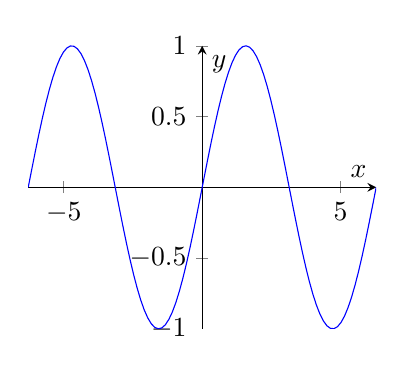
\begin{tikzpicture}
  \begin{axis}[
    xlabel=$x$,
    ylabel=$y$,
    width=6cm,
    axis lines=middle,
    domain=-2*pi:2*pi, % Set the domain for x-axis values
    samples=100 % Number of samples to plot
    ]
    % Plot the sine function
    \addplot[blue,mark=none] {sin(deg(x))};
  \end{axis}
\end{tikzpicture}
\hspace{2cm}
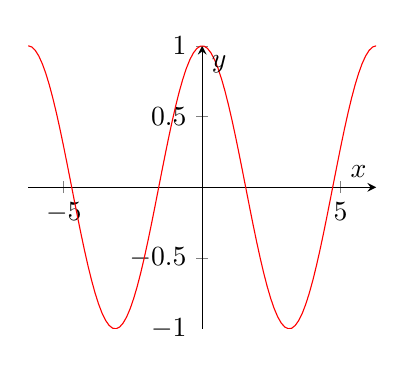
\begin{tikzpicture}
  \begin{axis}[
    xlabel=$x$,
    ylabel=$y$,
    width=6cm,
    axis lines=middle,
    domain=-2*pi:2*pi, % Set the domain for x-axis values
    samples=100 % Number of samples to plot
    ]
    % Plot the cosine function
    \addplot[red,mark=none] {cos(deg(x))};
  \end{axis}
\end{tikzpicture}
\end{center}

\subsection{General Sine and Cosine Functions}

Now, knowing how to graph the parent sine and cosine functions, we can take a look at more general forms of them. The general form of a sine function is as follows:

\[ f(x) = A\sin(b(x-h))+k \]

The constants $A, b, h,$ and $k$ all perform transformations on the parent function. 

$A$ vertically scales the wave, changing the maximum and minimum value of the function from $\pm 1$. $A$ is also known as the \textbf{amplitude}. 

$b$ changes the period of the wave from $2\pi$ to $\frac{2\pi}{b}$, essentially compressing or stretching the waves like a spring. $b$ is also known as the \textbf{angular frequency}.

Finally, $h$ and $k$ shift the wave horizontally and vertically, respectively.

The general form of a cosine function is the same as that of a sine function, only replacing $\sin$ with $\cos$. The transformation constants have the same effects on a cosine wave as they do on a sine wave.

\subsection{Other Trigonometric Functions}

The same logic and techniques can be applied to graph $\tan x$ and other trigonometric functions, such as the reciprocal functions $\csc x$, $\sec x$, and $\cot x$: determine the key points of the graph, as well as discontinuities if there are any, and draw a curve to connect the points. 

\section{Inverse Trigonometric Functions}

Previously, we learned that the inverse of a function is only a function if the original function passes the horizontal line test. Obviously, sine and cosine do not pass the horizontal line test. However, if we restrict the domain of sine and cosine to span only half of one period, it does pass the horizontal line test. This is shown below:

\begin{center}
\begin{tikzpicture}
  \begin{axis}[
    xlabel=$x$,
    ylabel=$y$,
    width=6cm,
    axis lines=middle,
    domain=-0.5*pi:0.5*pi, % Set the domain for x-axis values
    samples=100 % Number of samples to plot
    ]
    % Plot the sine function
    \addplot[blue,mark=none] {sin(deg(x))};
  \end{axis}
\end{tikzpicture}
\hspace{2cm}
\begin{tikzpicture}
  \begin{axis}[
    xlabel=$x$,
    ylabel=$y$,
    width=6cm,
    axis lines=middle,
    domain=-0:pi, % Set the domain for x-axis values
    samples=100 % Number of samples to plot
    ]
    % Plot the cosine function
    \addplot[red,mark=none] {cos(deg(x))};
  \end{axis}
\end{tikzpicture}
\end{center}

The restricted domain of sine is $[-\frac{\pi}{2}, \frac{pi}{2}]$, and the restricted domain of cosine is $[0, \pi]$. These domains span half of one period or half of the unit circle, but as can be seen, the resulting range spans all of $[-1, 1]$. Therefore, we can now define inverse functions of sine and cosine: 

\[\sin^{-1}(x) = \arcsin(x), \,\, \cos^{-1}(x) = \arccos(x) \]

The ranges of arcsine and arccosine are $[-\frac{\pi}{2}, \frac{\pi}{2}]$ and $[0, \pi]$, respectively. The domain of both is $[-1, 1]$.

Tangent also has an inverse function:

\[\tan^{-1}(x) = \arctan(x) \]

Unlike the bounded sine and cosine functions, the tangent function can take on any real value. Thus the inverse tangent function, arctangent, is defined for all real numbers. However, in order for arctangent to pass the vertical line test, we must truncate the original tangent function as we did previously. Therefore, the range of arctangent is reduced to $[-\frac{\pi}{2}, \frac{pi}{2}]$.

\end{document}